 \documentclass[a4paper, 11pt]{article}
\usepackage[utf8]{inputenc} 
\usepackage[T1]{fontenc}
%\usepackage{lmodern}
\usepackage{graphicx}
\usepackage[french]{babel}
\usepackage[left=2cm,right=2cm,top=1.5cm,bottom=2cm]{geometry}
\usepackage{fancyhdr}
\usepackage{amsmath,amsfonts,amssymb}
\usepackage{lastpage}
\usepackage{times}
%\usepackage[dvips]{graphicx}
\usepackage{epsfig}
\usepackage{amsmath}
%\usepackage{pgf,pgfarrows,pgfautomata,pgfheaps,pgfnodes,pgfshade}
\usepackage[useregional]{datetime2}
%\usepackage[amsmath]{maxiplot}

\usepackage{xcolor, soul}
%\sethlcolor{green}

\usepackage{tikz,tkz-tab}
\usepackage{tabularx}

\usepackage{moreverb}
\usepackage{hyperref}

\usepackage{makeidx} 
\makeindex

\usepackage{multicol}
\usepackage[tikz]{bclogo}
\usepackage{array}

\usepackage[shortlabels]{enumitem}
%\setlist[itemize,1]{label=$\star$}
\setlist[itemize,1]{label=\textbullet}
\setlist[itemize,2]{label=$\diamondsuit$} 

\renewcommand{\headrulewidth}{0.0pt}
\renewcommand{\footrulewidth}{0.5pt}

\setlength{\parindent}{0pt}

\newcounter{num}
\renewcommand{\thenum}{\Roman{num}}
\newcommand{\exo}{\addtocounter{num}{1}{\noindent \textbf{Exercice~\thenum~:}}}
\newenvironment{exercice}{\exo}{\vspace{0.4cm}}
\newcommand{\version}{2.0}

\begin{document}

\pagestyle{fancy} \lhead{} \chead{} \rhead{} 
\rfoot{\small{{\thepage/\pageref{LastPage}}}} 
\cfoot{Version \version} 
\lfoot{Logiciel mac2texpdf2}

\setcounter{tocdepth}{2}
\renewcommand*{\contentsname}{Sommaire}

\fbox{\makebox[\textwidth][c]{\textbf{
\LARGE Documentation du logiciel mac2texpdf2
}}}

\begin{center}
{\large \textbf{Version \version{} du \today} \\
Auteur : Michel Gosse, michel.gosse@free.fr}
\end{center}

 
%\tableofcontents

\section*{Présentation}
Ce logiciel est un utilitaire permettant la saisie de commandes pour le logiciel Maxima (soit en les saisissant, soit après un copier/coller) qui génère un fichier PDF comprenant les commandes saisies ainsi que les résultats calculés par Maxima. Il permet en outre l'exportation du fichier \LaTeX{} utilisé pour la production du PDF ainsi que des images du document dans un dossier choisi par l'utilisateur.

\subsection*{Copies d'écran}

\begin{figure}[ht]
  \centering
  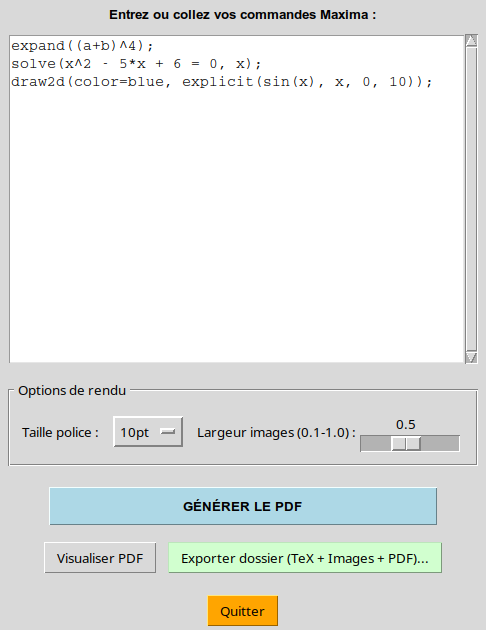
\includegraphics[width=0.45\textwidth]{img1mac2tex.png}% 
  \hspace{0.05\textwidth}%
  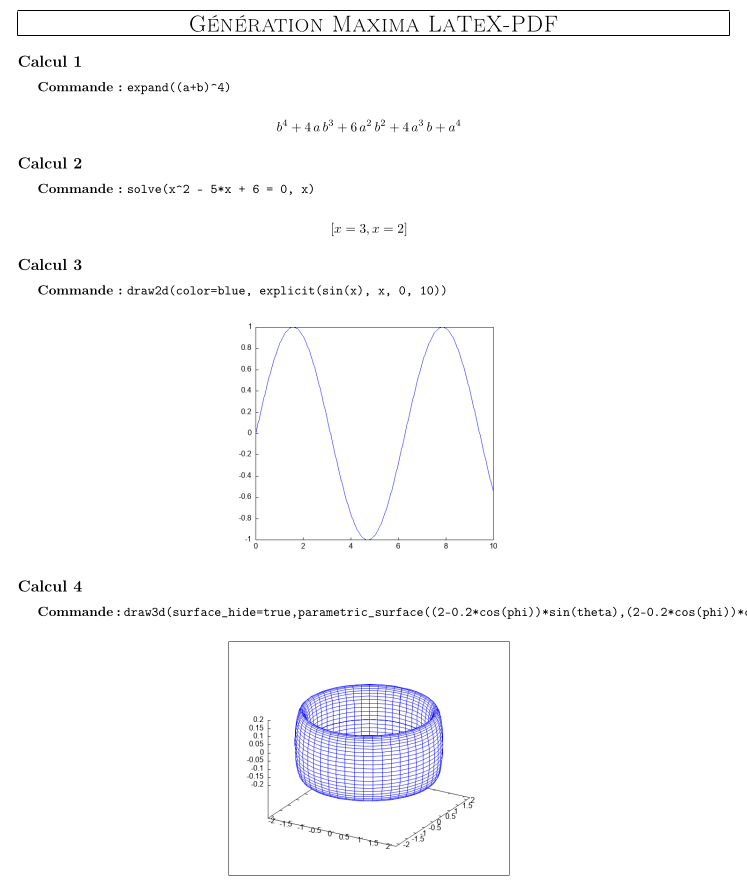
\includegraphics[width=0.45\textwidth]{img3mac2tex.png}
\end{figure}

\subsection*{Principe du logiciel}

Le logiciel envoie les commandes au logiciel de calcul formel Maxima (ligne par ligne), qui les exécute et renvoie le résultat en \LaTeX{}. Le logiciel récupère ces données et les met en page dans un document \LaTeX{} qui est ensuite compilé avec pdflatex. Il s'agit d'un script Python, qui est aussi disponible sous la forme d'un exécutable pour Windows ou pour Linux.

\subsection*{Comparaison avec wxMaxima}

Cet utilitaire est un outil léger et rapide qui permet d'obtenir rapidement un document de bonne qualité comprenant les résultats calculés par Maxima de commandes entrées par l'utilsateur (au format PDF ou \LaTeX{}). Il n'offre pas la puissance de wxMaxima et n'est pas adapté pour résoudre des exercices complexes.

\subsection*{Pré-requis}

Pour fonctionner, le logiciel nécessite :
\begin{enumerate}
\item le logiciel Maxima
\item le logiciel Gnuplot 
\item une distribution \LaTeX{} incluant les packages suivants : xcolor, listings, datetime2, babel, geometry, fancyhdr, lastpage, graphicx, mathtools, amsmath, amsfonts, asmssymb
\item si on souhaite utiliser la version source (le script Python), alors il faut aussi que Python soit installé sur l'ordinateur.
\end{enumerate} 

\emph{Les différentes installations sont détaillés par système d'exploitation ci-dessous.}

\section*{Installation pour Windows}

\subsection*{Etape 1 : installer Maxima et mettre Maxima dans le PATH}
$\blacktriangleright$ Télécharger et installer Maxima (version 5.49.0) :
\begin{center}
\href{https://sourceforge.net/projects/maxima/files/Maxima-Windows/5.49.0-Windows/}
{https://sourceforge.net/projects/maxima/files/Maxima-Windows/5.49.0-Windows/}
\end{center}

$\blacktriangleright$ Modifier les variable d'environnement :
\begin{enumerate}
\item Ouvrir les paramètres : Touche Windows + I
\item Aller dans Système → À propos.
\item Cliquer sur Paramètres avancés du système (ou Paramètres système avancés).
\item Dans la fenêtre qui s’ouvre, cliquer sur le bouton Variables d’environnement… en bas
\item Choisir PATH et modifier
\item Rajouter les deux lignes en fin du texte \\
C:\textbackslash maxima-5.49.01 \textbackslash bin \\
C:\textbackslash maxima-5.49.01 \textbackslash gnuplot \textbackslash bin
\item Valider avec OK plusieurs fois pour fermer toutes les fenêtres
\end{enumerate}

\textit{Remarque} : le logiciel Gnuplot est installé automatiquement en même temps que Maxima.

\subsection*{Etape 2 : Intallation d'une distribution \LaTeX{}}
Si \LaTeX est installé, vérifier que les packages  xcolor, listings, datetime2, babel, geometry, fancyhdr, lastpage, graphicx, mathtools, amsmath, amsfonts, asmssymb sont bien installés.

Sinon, télécharger la distribution Texlive et l'installer (elle installe automatiquement tous les packages requis et modifie le PATH directement) :

\begin{center}
\href{https://tug.org/texlive/windows.html}{https://tug.org/texlive/windows.html}
\end{center}

\subsection*{Etape 3 facultative : installation de Python}

Si vous souhaitez utiliserle script Python et non pas l'exécutable, il faut installer Python (l'installation l'ajoute aussi dans le PATH automatiquement).

\begin{center}
\href{https://www.python.org/downloads/windows/}{https://www.python.org/downloads/windows/}
\end{center}

\subsection*{Etape 4 : Télécharger le logiciel mac2texpdf2.exe}
Télécharger la version Windows sur la page :

\begin{center}
\href{https://maxima-french-doc.fr/interfaces/}{https://maxima-french-doc.fr/interfaces/}
\end{center}
Il reste à dézipper le fichier et à double-cliquer sur l'exécutable Windows ainsi récupéré (il s'appelle mac2texpdf2-w.exe).

Windows émet un avertisement indiquant que le logiciel n'est pas certifié. Pour le lancer, il faut accepter de lancer un logiciel inconnu...

\textbf{Alternative avec Python : télécharger le script Python mac2texpdf2-w.py}

Une fois dézippé, il faut ouvrir une invite de commandes, se placer dans le dossier contenant le fichier python, et taper la commande :
\textit{python mac2texpdf2-w.py}

\section*{Installation pour Linux}

\subsection*{Etape 1 : Installer Maxima}
Si le logiciel  n'est pas installé, on peut soit l'installer via le gestionnaire de package de sa distribution, ou le télécharger à partir de la page :

\begin{center}
\href{https://sourceforge.net/projects/maxima/files/Maxima-Linux/5.49.0-Linux/}{https://sourceforge.net/projects/maxima/files/Maxima-Linux/5.49.0-Linux/}
\end{center}
Le PATH est ajouté automatiquement (contrairement à windows).

\subsection*{Etape 2 : Installer \LaTeX{}}
A faire avec le gestionnaire de packages de sa distribution. On fera une installation complète pour avoir tous les packages requis. Sinon, ils sont contenus dans le package texlive-latex-extra.

\subsection*{Etape 3: Facultatif : installation de Python}
Si l'on souhaite utiliser le script Python et non pas le binaire, on installe Python via le gestionnaire de packages de sa distribution.

\subsection*{Etape 4 : Télécharger le logiciel mac2texpdf2.bin}
Télécharger la version Linux sur la page :

\begin{center}
\href{https://maxima-french-doc.fr/interfaces/}{https://maxima-french-doc.fr/interfaces/}
\end{center}
Il reste à dézipper le fichier et à double-cliquer sur le binaire Linux ainsi récupéré (il s'appelle mac2texpdf2.bin).

\textbf{Alternative avec Python : télécharger le script Python mac2texpdf2.py}

Une fois dézippé, il faut ouvrir un terminal, se placer dans le dossier contenant le fichier python, et taper la commande :
\textit{python3 mac2texpdf2.py}


\section*{Utilisation de mac2texpdf2}

Le fonctionnement est très simple :
\begin{itemize}
\item On entre dans la zone de texte une suite de commandes Maxima. \emph{Chaque commande est sur une seule ligne et doit se terminer par un ;}
\item On choisit la taille de la police pour le PDF qui sera généré. S'il y a des graphiques, on choisit l'échelle pour les graphiques (entre 0 et 1).
\item On clique sur Générer le PDF
\item Il reste à cliquer sur Voir le PDF. 
\item Si on souhaite récupérer le PDF et le fichier \LaTeX{} correspondant (avec les images du document), on clique sur le bouton exporter dossier.
\end{itemize}

\subsection*{Quelques points d'attention}

\begin{itemize}
\item pour les graphiques, on utilisera les commandes draw2d et draw3d. Les commandes wxdraw2d et wsdraw3d sont spécifiques au logiciel wxMaxima et ne sont pas reconnues par Maxima qui les ignore.
\item les entrées/sorties de Maxima n'étant pas numérotées par le logiciel mac2texpdf2, on ne peut pas utiliser \% pour désigner le résultat précédent.
Par exemple :
\begin{verbatim}
solve(a*x^2-1=0,x);
subst(5,a,%);
\end{verbatim}
ne fonctionne pas. Il faut à la place nommer chaque résultat pour l'utiliser ultérieurement :
\begin{verbatim}
eq:solve(a*x^2-1=0,x);
subst(5,a,eq);
\end{verbatim}
\end{itemize}

\section*{Liens et références }

\subsection*{Documentation sur Maxima}
\href{https://maxima-french-doc.fr/documentation/}{https://maxima-french-doc.fr/documentation/}

\subsection*{Page du logiciel mac2texpdf2}
\href{https://maxima-french-doc.fr/interfaces/}{https://maxima-french-doc.fr/interfaces/}

\subsection*{Site du développement du logiciel mac2texpdf2}
Le logiciel est en développement dans un dépot github :

\href{https://github.com/michelprog59/mac2texpdf2}{https://github.com/michelprog59/mac2texpdf2}

\subsection*{Licence et contact}
Le logiciel est distribué Distribué sous licence GNU GENERAL PUBLIC LICENSE (GPL) v3.0 et peut être utilisé et modifié librement.

Pour toutes demandes d'évolution ou de signalement de bugs, on peut soit le faire directement sur github, soit m'envoyer un mail à michel.gosse@free.fr

\end{document}